\documentclass[10pt, conference, letterpaper]{IEEEtran}
\usepackage{cite}
\usepackage{xcolor,soul,framed}
\usepackage{amsmath,amsthm,amssymb,amsfonts}
\usepackage{algorithmic}
\usepackage{graphicx}
\usepackage{color, soul}
\usepackage{algorithm, algorithmic}
\usepackage[utf8]{inputenc}
\usepackage[english]{babel}
\usepackage{mathtools}
\graphicspath{ {./images/} }

%---------------------------------------------------------------%
\newtheorem{definition}{Definition}
\newtheorem{assumption}{Assumption}
\newtheorem{problem}{Problem}
\newtheorem{lemma}{Lemma}
\newtheorem{remark}{Remark}
\newtheorem{theorem}{Theorem}
\newtheorem{corollary}{Corollary}
\newtheorem{example}{Example}
\newcommand{\eq}{=}
\newcommand{\domZ}{\mathbb{Z}_{*}}
\newcommand{\vecOne}{\mathbf{1}}
\newcommand{\ind}{\mathbf{I}}
\newcommand{\mat}{\mathbf}
\newcommand{\Poisson}{\text{Poisson}}
\newcommand{\define}{\triangleq}
\newcommand{\leadto}{\Rightarrow}
\newcommand{\vecG}{\boldsymbol}
\renewcommand{\vec}{\mathbf}
\DeclarePairedDelimiter{\set}{\{}{\}}
\DeclarePairedDelimiter{\norm}{|}{|}
\DeclarePairedDelimiter{\Inorm}{\|}{\|_1}
\DeclarePairedDelimiter{\Paren}{\bigg(}{\bigg)}
\DeclarePairedDelimiter{\Bracket}{\bigg[}{\bigg]}
\DeclarePairedDelimiter{\Brace}{\bigg\{}{\bigg\}}
%---------------------------------------------------------------%
\newcommand{\apSet}{\mathcal{K}}
\newcommand{\esSet}{\mathcal{M}}
\newcommand{\jSpace}{\mathcal{J}}
\newcommand{\Stat}{\mathbf{S}}
\newcommand{\Obsv}{\mathcal{Y}}
\newcommand{\Policy}{\boldsymbol{\Omega}}
\newcommand{\BPolicy}{\Policy} %{\bar{\Policy}}
\newcommand{\ASpace}{\mathbf{A}}
%---------------------------------------------------------------%

\begin{document}
    %=============================== TITLE ===============================%
    \title{
        Obsolete Partial Information-based Distributed Online Job Dispatching in Edge Computing System
    }
    % \author{
    %     \IEEEauthorblockN{
    %         Yuncong Hong\IEEEauthorrefmark{1}\IEEEauthorrefmark{2},
    %         Zhenhua Han\IEEEauthorrefmark{2}
    %         Rui Wang\IEEEauthorrefmark{1},
    %         Haisheng Tan\IEEEauthorrefmark{3},
    %         Francis C.M. Lau\IEEEauthorrefmark{2}
    %     }
    %     \IEEEauthorblockA{
    %         \IEEEauthorrefmark{1}Southern University of Science and Technology, P.R. China,
    %         \IEEEauthorrefmark{2}The University of Hong Kong, Hong Kong,\\
    %         \IEEEauthorrefmark{3}University of Science and Technology of China, P.R. China
    %     }
    % }
    \maketitle

    %============================== ABSTRACT ==============================%
    \begin{abstract}
        \label{sec:abstract}
        Edge computing is believed to be the solid solution for time-sensitive big data real-time calculation. The cooperation among edge servers in the system usually causes in-effective task scheduling due to obsolete information sharing which is hard to tackle.
        In this work, we formulate the problem with job dispatching in distributed Edge Computing system, and identify the difficulty exists in cooperation among AP nodes (Access Points) and ES nodes (Edge Servers) with delayed information. We design the broadcast information sharing scheme in the system and formulate the corresponding problem into a MDP problem. The value function approximation and one-step policy iteration method is adopted to obtain a sub-optimal dispatching policy whose performance can be bounded analytically.
    \end{abstract}

    % \begin{IEEEkeywords}
    %     Edge Computing, Job Dispatch, Delayed Information, Collective Observability, Distributed Multi-agent MDP
    % \end{IEEEkeywords}

    %============================ INTRODUCTION ============================%
    \begin{section}{INTRODUCTION}
        \label{sec:introduction}
        Edge Computation is believed to be a promising technology for solving increasingly communication congestion in backbone network.
        (Rich-media tasks are delay-sensitive).
        \cite{Naha2018} is a survey about fog computing in latency-aware computing in IoT, and investigate numerous proposed computing architecture.

        Related works on job dispatching on scheduling in edge computing, mostly with centralized agent to apply action and seldom take delayed information impact into consideration.
        There are some previous works on jobs scheduling strategies under the scenario of edge computation, together with joint optimization job dispatching and resource allocation:
        \begin{itemize}
            \item \cite{Zheng2019} is a work considering maximizing the long-term utility in MEC offloading policy, and formulating the problem with MDP solved with Q-learning (However, it's applied with a centralized controller which would suffer from communication overhead, and without performance guarantee);
            \item \cite{Du2018} propose an offline algorithm with MINLP (Mixed-Integer Nonlinear Programming) problem formulation, considering min-max fairness guarantee in computation offloading and computation resource allocation in fog/edge computing scenario (However, with only one edge and one cloud node considered);
            \item \cite{Alameddine2019} is a work considering task offloading, scheduling and resource allocation joint optimization with Benders Decomposition (However, delay information is previous defined);
            \item \cite{Fan2017} considers cooperation of multiple MEC-BSs of computation offloading to other MEC-BSs (However, it doesn't consider the offloading utility impact on other MEC-BSs, i.e. only optimize for one BSs in the cluster).
        \end{itemize}
        
        Different from the previous referred works, which only consider optimization for one agent in system or using centralized agent for decision making, we focus on the impact of out-of-dated information on decision making in multiple agents distributed cooperation.
        Due to frequent jobs releasing from users and uncertainty of jobs uploading time to servers, the obsolete information is inevitable in a purely distributed system.
        This information sharing delay would cause severe mis-estimate for job dispatching decision making, and thus it will be hard to guarantee the cooperation among individual agents.
        Moreover, the information sharing delay is often un-deterministic due to shared under-laid network topology, and offensively sharing strategy would cause network congestion to other normal functions.

        As what we have learned for now, there are very limited discussions on this topic:
        \begin{itemize}
            \item The earliest works entangling with out-of-dated information we could find is \cite{ref-01} (cited 167 times). In this work, the single agent is assumed not able to observe the global state, and thus they need communication to establish cooperation by sharing limited information. The agent considers communication as extra action to synchronize the states and thus incurs extra cost (However, the communication is without delay, thus converted into POMDP problem; criticize with impractical);
            \item The other work \cite{ref-02} considers continuous state observation with constant or stochastic delay with single agent;
            \item One researcher published a series of paper on this topic \cite{Lyu2017,Lyu2018,Lyu2018a,Lyu2018b}.
                \cite{Lyu2017} is work considering \emph{partial out-of-date knowledge} optimization in IoT computing scenario, with Lyapunov optimization;
                \text{[delay-sensitive, ToC]} \cite{Lyu2018} identify that task admission is critical to delay-sensitive applications in mobile edge computing, and proposes an (1-$\epsilon$)-approximation algorithm
                \text{[foggy, fully distributed online]} \cite{Lyu2018a} is a work fully distributed online optimization to minimize the time-average cost and achieve asymptotic optimality over infinite time;
                \cite{Lyu2018b} try to establish cooperation among selfish devices in fog computing, and out-of-date information is blamed for optimality gap but proved to asymptotically diminish with the proposed algorithm (However, the out-dated information is considered with limited effect);
        \end{itemize}

        % Service Placement Scenario:
        % \begin{itemize}
        %     \item \cite{Rodrigues2017} is a work on minimizing service delay in mobile edge computing;
        %     \item \cite{Yang2016} is a work considering services placement and requests dispatching on edge servers, and leverage users' pattern to predict "service cache" for online decision making;
        %     \item \cite{Chen2018} is a work with SDN on task offloading and battery life saving, and solve the NLP problem with two sub-problems;
        % \end{itemize}
        % Using Game Theory:
        % \begin{itemize}
        %     \item \cite{yang2018} and \cite{Josilo2019a} considers distributed computation offloading game;
        %     \item \cite{Liu2018} is a work considering minimize users' power consumption with Lyapunov optimization and matching theory;
        %     \item \cite{Dinh2018} considers distributed multi-user offloading in wireless channel with selfish EPG (exact potential game);
        %     \item \cite{Josilo2019} considers selfish offloading to achieve Nash equilibrium;
        %     \item \cite{Chen2016} is a work considering multi-user computation offloading with multi-channel contention, and adopt game theory approach to achieve Nash equilibrium with upper bound of convergence time;
        %     \item \cite{Zhang2018} considers multi-user offloading under transmit power decision and user association decision;
        % \end{itemize}
        % System Work:
        % \begin{itemize}
        %     \item \cite{Yu2018} is a system work published in ToMC, presents a framework to minimize remote execution overhead, and carry out real system experiments using large-scale data from cellular network provider;
        %     \item \cite{Wang2018} is a system work published in IEEE Access, considers the mobility of mobile users in limited coverage solved with service migration and handover, and propose a framework;
        % \end{itemize}

        In this article, we consider there are Access Points (AP) in this network to connect the User Equipment (UE) and the Edge Servers (ES).
        The computation jobs would be released from UEs and the dispatching decisions are determined distributed on each AP nodes as depicted in Fig.\ref{fig:system}.
        The information sharing scheme is proposed in this article with synchronized broadcast design. With the help of this scheme, we could immediately apply the job dispatching decision based on obsolete information, with some prior stochastic knowledge of global system.
        Our contributions are summarized as follows.
        \begin{itemize}
            \item To our best knowledge, we are the first work to propose the MDP framework making use of obsolete information in edge computing system. With shared prior stochastic knowledge about broadcast latency and uploading delay, the distributed agent could come to consensus on optimal policy adopting globally;
            \item We propose a global state MDP formulation to characterize the multiple-agent problem, i.e. single agent would consider multiple-agent decision optimality to achieve cooperation.
            We with adopt value function approximation to reduce the traditional algorithm complexity, and come up with performance guarantee performance bound.
        \end{itemize}

        \hl{The remainder of this paper is organized as follows.}
        In Sec.II, system model.
        In Sec.III, problem formulation.
        In Sec.IV, we introduce low-complexity MDP algorithm.
        In Sec.V, evaluation.
        In Sec.VI, conclusion.
    \end{section}

    %============================ SYSTEM MODEL ============================%
    \begin{section}{SYSTEM MODEL}
        \label{sec:model}
        \begin{subsection}{Network Model}
            We have Access Points (AP) and Edge Servers (ES) denoted as $\apSet \define \set{1,\dots,K}$ and $\mathcal{M} \define \set{1,\dots,M}$ respectively in our MEC (mobile edge computing) system depicted in Fig. \ref{fig:system}. In this system, we adopt the same timing mechanism at both AP and ES side with a minimum \emph{timeslot} lasting for $\tau$ seconds.

            \begin{figure}[ht]
                \centering
                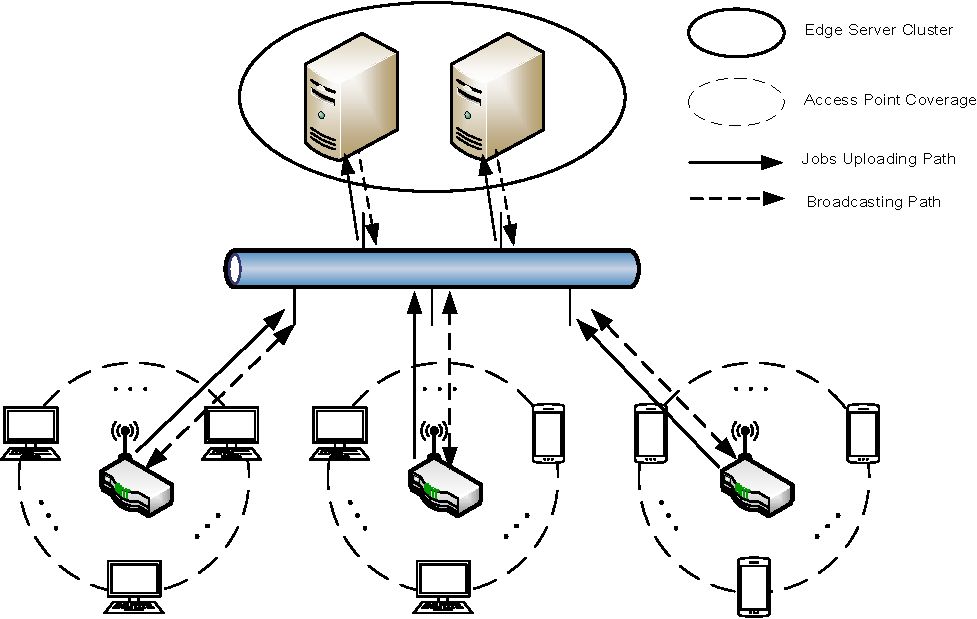
\includegraphics[width=0.45\textwidth]{system-model.pdf}
                \caption{The Illustration of MEC System Model}
                \label{fig:system}
            \end{figure}

            The User Equipment (UE) would offload the computation jobs on demand to the AP it connect.
            We consider some types of jobs are supported on edge servers with Virtual Machine (VM) resources. The job space is denoted as $\jSpace \define \set{1,\dots, J}$, and jobs type distribution on each AP node follows the same distribution over $\jSpace$.
            % which is obtained by statistics and denoted as $p_j \define \Pr\{\text{"j-type arrival"}\}$, where $\sum_{j\in\jSpace} p_j=1$.
            Thus the job arrival process on $k$-th AP ($\forall k\in\apSet$) is compounded of the job arrivals from all UE connected, which follows the assumption as:
            \begin{assumption}[Job Arrival Process for AP]
                The $j$-type job arrival distribution for $k$-th AP is denoted as $A_{k,j}$, which is independent and identically distributed (i.i.d) over each timeslot as $A_{k,j}$ following Poisson Point Process with intensity $\lambda_{k,j}$ ($\lambda_{k,j} > 0$). Thus average arrival rate of $j$-type jobs on $k$-th AP is $\mathbb{E}[A_{k,j}]=\lambda_{k,j}$, which implies that the occurrence average number of jobs in one timeslot would be $\lambda_{k,j}\tau$, .
            \end{assumption}

            The AP itself is assumed with no computation capability, and thus it need to further dispatch those jobs to the edge servers.
            The jobs arrival in each timeslot on AP will be immediately dispatched to edge servers.
            The corresponding uploading delay of one job is \emph{deterministic and job-type dependent} over one AP-ES link, which is denoted as $u_{k,m}(j)$ from $k$-th AP to $m$-th ES ($\forall k\in\apSet, \forall m\in\esSet$).

            After arrival on edge servers, the jobs will join computation queue with the supported VM.
            Each VM is considered running parallel without resource contention, and the jobs scheduling for each VM is with a single queue following \emph{FCFS} (First-Come-First-Serve).
            {\color{red}The maximum queue length is set to discourage too many jobs pending on edge servers and is denoted as $L_Q$. The job submission over the limit will be rejected and announce the AP where the job is from.}

            {\color{red}For jobs processing on edge servers, we adopt \emph{unrelated machines} assumption in \cite{tan-online}, where the job processing time on different servers are machine dependent and variant of resource or VM (virtual machine) constraints.
            Moreover, we have $l_{m,j}$ to denote the processing time for $j$-type job on $m$-th edge serer following some distribution, whose largest processing time is bounded by $l_C$.}
            For convenience, we assign type of jobs on edge servers which have no VM resource available with \emph{infinity} processing time, and this kind of dispatching possibility will be rejected at the AP side.
        \end{subsection}

        \begin{subsection}{Information-Sharing Broadcast Model}
            As there is no centralized agent to distribute dispatching decisions to each AP node, an efficient information sharing scheme is needed to help collect global information and establish cooperation among standalone nodes.
            In this paper, the proposed sharing scheme is designed via periodic broadcasting, where all the AP and ES nodes in the system should broadcast their system related information with a same period interval as $t_B$. More specifically, the broadcasting is applied in a synchronized way that all the nodes start to broadcast at the start of same timeslot and repeat broadcasting after the same periodic interval $t_B$. We call each periodic point of broadcasting as \emph{broadcast point} and denote the $i$-th broadcast with $t_i$ where,
            \begin{align}
                t_i = i \cdot t_B, i=0,1,2,\dots
            \end{align}
            For $i$-th \emph{broadcast point}, the composed broadcast information from all the AP and ES nodes, and the corresponding information is listed as follows.
            \begin{itemize}
                \item The $k$-th AP ($\forall k\in\apSet$) contains information $\mat{R}_k(i) \define (r^{(k)}_{m,j}(i))_{\set{m\in\esSet,j\in\jSpace}}$, where $r^{(k)}_{m,j}(i)$ denotes the remaining number of $j$-type jobs in uploading to $m$-th ES at time $t_i$; and we have $\vec{r}^{(k)}_{m} \define (r^{(k)}_{m,j}(i))_{j\in\jSpace}$ to denote the rows in $\vec{R}_k(i)$;
                \item The $m$-th ES ($\forall m\in\esSet$) contains information $\vec{Q}_m(i) \define \set{Q_{m,j}(i)|\forall j\in\jSpace}$ to denote the computation queues for different job types, where $Q_{m,j}(i) \define (q_{m,j}(i), \delta_{m,j}(i))$ to characterize the $j$-type FIFO queue on $m$-th ES; $q_{m,j}(i)$ denotes the number of $j$-type job queueing on $m$-th ES, and $\delta_{m,j}(i)$ denotes the remaining processing time for last job.
            \end{itemize}
            Thus the composed broadcasting information is denoted as:
            \begin{align}
                \Obsv_i \define
                        \Brace{
                            \set{\mat{R}_{k}(i)|\forall k\in\apSet},
                            \set{\vec{Q}_m(i)|\forall m\in\esSet}
                        },
            \end{align}
            where $\Obsv_i$ is a set of global information of $i$-th broadcast. And it's actually the global system states at $t_i$.

            We consider different AP nodes would receive partial broadcast information at different time points in one broadcast interval.
            Let $d^{(p)}_{k,k'}$ denotes the broadcast delay between two AP nodes from $k'$-th AP to $k$-th AP ($\forall k,k'\in\apSet$); let $d^{(s)}_{k,m}$ denotes the broadcast delay between AP and ES node from $m$-th ES to $k$-th AP ($\forall k\in\apSet,\forall m\in\esSet$).
            Then we denote the latency for $k$-th AP receives broadcast information from other nodes (including all ES nodes and other AP nodes) as \emph{Maximum Broadcast Latency}.
            \begin{definition}[Maximum Broadcast Latency]
                The maximum broadcast latency is the time when AP receives whole broadcast information with respect to the broadcast point. For $k$-th AP ($\forall k\in\apSet$) the latency is defined as follows.
                \begin{align}
                    \hat{d}_{k} \define \max\Paren{ \set{d^{(p)}_{k,k'}, d^{(s)}_{k,m}|\forall k' \neq k \in\apSet, \forall m\in\esSet} }
                \end{align}
                Without loss of generality, we sort the index of AP set $\apSet$ according to the corresponding maximum delay that the global information is received, i.e. $\hat{d}_{1} \leq \hat{d}_{2} \leq \dots \leq \hat{d}_{K}$. We will keep this assumption in the remaining of the article.
            \end{definition}
            {\color{red}
            Moreover, we implement the broadcast in a low-frequency way that the broadcast period is always larger than the maximum broadcast latency pulsing the maximum uploading delay, i.e. $t_B > \hat{d}_{k} + u_{k,m}(j)$ $(\forall k\in\apSet, \forall m\in\esSet, \forall j\in\jSpace)$.
            }

            {\color{red}
            Due to the introduced periodic broadcasting design and the information receiving latency, this kind of system is inherent of the structure that decisions are always made with obsolete and partial information.
            This implies that: if any agents change its decision with respect to newly-arrival broadcast information, it will disturb other agents' decisions from cooperation due to different information of system states.
            Thus, it's unacceptable to update agents' policy only when the agents all come up with exactly same information.
            So we consider \emph{partial information}-based dispatching decision making to adapt to new information as soon as possible.
            }
            
            In the problem formulation section, we will show that we could leverage obsolete and partial information to improve the policy applied on different AP nodes. Furthermore, with the help of algorithm design we could prove that our improved policy is with analytical performance bound under MDP framework.
        \end{subsection}
    \end{section}

    %============================ FORMULATION =============================%
    \begin{section}{PROBLEM FORMULATION}
        \label{sec:formulation}
        In this section, we formulate the standard MDP problem with respect to global system states and jobs dispatching policy of which is compounded of all AP nodes in this MEC system.
        Given the fact that AP nodes would obtain global states update only after \emph{Update Latency} in each broadcast interval, the formulated MDP problem is composed of two adjacent broadcast interval with obsolete information and updated information.
        As we allow policy update over partial obsolete information, the formulated MDP problem is further split into two sub-problem leveraging same problem structure. The structure would lead to performance improvement guarantee with the proposed distributed algorithm.
        Then we show that the solution for all AP nodes suffers from curse of dimensionality and a low-complexity solution is needed.

        \begin{subsection}{System State and Dispatching Policy}
            The system states is selected based on the nature that $k$-th AP comes up with complete broadcast information only after its corresponding \emph{Update Latency} in the broadcast interval.
            The relative difference between broadcast point and the update time point is depicted in Fig. \ref{fig:brd-trans}.
            \begin{definition}[System State]
                The system state at $i$-th broadcast point is denoted as $\Stat_i \define (\Obsv_{i-2}, \Obsv_{i-1}, \Obsv_{i}), (i=1,2,\dots)$, where $\Obsv_{-1}=\Obsv_{0} =\Phi$ denotes the empty system state.
                $\Obsv_{i}$ denotes updated information after receiving global broadcasting information, $\Obsv_{i-1}$ denotes the partial stale information, and $\Obsv_{i-2}$ denotes the more stale information which have impact on transition function with respect to $\Obsv_{i-2}$.
            \end{definition}

            \begin{figure}[ht]
                \centering
                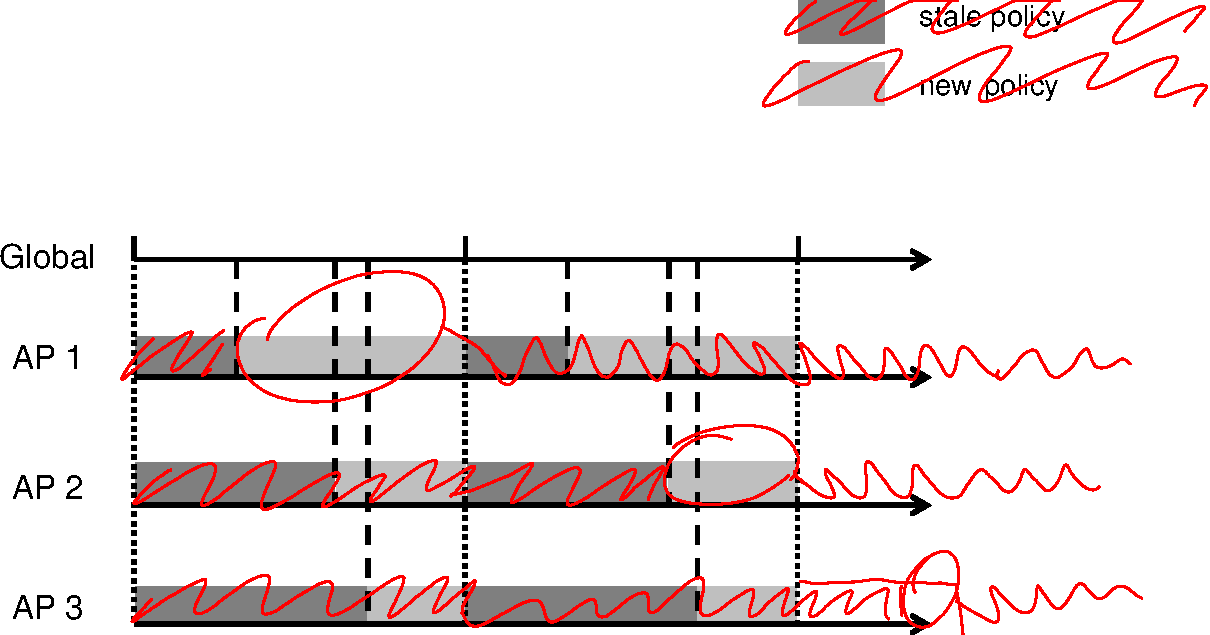
\includegraphics[width=0.45\textwidth]{brd-trans.pdf}
                \caption{Global System Transition with Partial Information-based Dispatching Decision}
                \label{fig:brd-trans}
            \end{figure}

            The \emph{dispatching policy} is applied over arrival jobs in each timeslot on each AP, and thus \emph{dispatching action space} is defined as $\mathbf{A}: (j, m) \in \jSpace \times \esSet$ where $(j, m)$ denotes the action that $j$-type job should be uploaded to $m$-th ES.
            \begin{definition}[Update Time Points]
                For $k$-th AP ($\forall k\in\apSet$), partial updates firstly and then consensus update, which is defined as follows.
                \begin{itemize}
                    \item Partial Update Point: The AP nodes will update their own policy when the corresponding \emph{Maximum Broadcast Latency} is achieved, and awareness of the previous policy change for the AP nodes receiving information before it;
                    \item Iterative Update Points: When reaching the ending of the broadcast interval, all the AP nodes would update the policy together;
                    this policy iteration is evaluated with no policy changes consideration in the following time in this interval;
                    this policy iteration is with partial information only with last interval, but not with information from this interval.
                \end{itemize}
            \end{definition}
            
            Based on the three stages of global system information defined in system state, the compounded global-wise policy of all AP nodes is defined as follows.
            \begin{definition}[Compounded Dispatching Policy]
                The compounded dispatching policy $\Policy(\Stat_{i})$ over $\Stat_{i}$ which is defined with three-stage broadcasting information which is given as follows.
                \begin{align}
                    \Policy(\Stat_{i}) \define \Bracket{
                        \Omega'(\Obsv_{i-2}), \Omega(\Obsv_{i-1}), \Omega'(\Obsv_{i-1}), \Omega(\Obsv_{i}),
                    }
                \end{align}
                where $\Omega'(\Obsv_i) \define [\tilde{\Omega}'_{1}(\Obsv_i), \dots, \tilde{\Omega}'_{K}(\Obsv_i)]$ denotes the policy applied at \emph{Partial Update Point} with obsolete partial information; and $\Omega(\Obsv_i) \define [\tilde{\Omega}_{1}(\Obsv_i), \dots, \tilde{\Omega}_{K}(\Obsv_i)]$ denotes the policy at \emph{Iterative Update Points} respectively, i.e. $k$-th AP ($\forall k\in\apSet$) would change its policy from $\tilde{\Omega}_{k}'(\Obsv_i)$ to $\tilde{\Omega}_{k}(\Obsv_{i+1})$ when receiving information $\Obsv_{i+1}$ while the others keep their own policy.
                
                Furthermore, the local policy for AP nodes is defined according to \emph{dispatching action space} as follows.
                \begin{align}
                    &\tilde{\Omega}_{k}(\Obsv_{i}) \define \set{\omega^{(i)}_{k,j}(m)|\forall j\in\jSpace, \forall m\in\esSet}
                    \;(\forall k\in\apSet)
                    \\
                    &\tilde{\Omega}'_{k}(\Obsv_{i}) \define \set{\omega'^{(i)}_{k,j}(m)|\forall j\in\jSpace, \forall m\in\esSet}
                    \;(\forall k\in\apSet),
                \end{align}
                where $\omega^{(i)}_{k,j}(m)$ denotes the deterministic dispatching policy that: when $k$-th AP with information $\Obsv_{i}$ after its iterative update point, it would then upload $j$-type job to $m$-th ES if and only if $\omega^{(i)}_{k,j}(m)=1$; $\tilde{\Omega}'_{k}(\Obsv_i)$ is for partial update point.
            \end{definition}

            More specifically, the multiple-phase of the policy $\tilde{\Omega}_k(\Obsv_i)$ at multiple \emph{iterative update points} are separated by \emph{Update Latency} $d_{k}$ for $k$-th AP ($k\in\apSet$). One vivid example of policy adaption phase is given as follows, the update rules of which will be elaborated in next sub-section.
            \begin{example}[Policy Phase Adaption]
                In the time interval $[t_{i}, t_{i+1}]$, $k$-th AP would adopt $\tilde{\Omega}_{k}'(\Obsv_{i-1})$ immediately after $t_i$, and adopt $\tilde{\Omega}_{k}(\Obsv_{i})$ after its corresponding iterative update points; then with $\tilde{\Omega}_{k}'(\Obsv_{i})$ at $t_{i+1}$ and repeat the process.
            \end{example}
        \end{subsection}

        \begin{subsection}{The Optimization Problem}
            We propose the jobs dispatching optimization problem with the target to minimize \emph{average response time} of all offloaded jobs in MEC system.
            The \emph{average response time} is composed of uploading time from $AP$ to $ES$, and queueing-and-service time on corresponding ES. According to \emph{Little's Law}, the average response time of all jobs is equally as average number of jobs in system.
            
            Due to the intrinsic property of periodic information broadcasting, we collect the cost for number counting at the pace of broadcasting interval which could be seems as sampling of original process based on timeslot scale.
            Besides the cost counted for job response time, we furthermore add penalty on jobs submission over its capacity limit when the over-limited jobs will be rejected at the end of current broadcast interval.
            Therefore, the cost function of this problem is given as follows.
            \begin{align}
                g\Paren{\Stat_{i}, \Policy(\Stat_{i})} \define& \sum_{k\in\apSet}\sum_{m\in\esSet} \Inorm{\vec{r}^{(k)}_{m}(i)} + \sum_{m\in\esSet}\sum_{j\in\jSpace}
                \nonumber\\
                &\Brace{
                    q_{m,j}(i) + \beta I[q_{m,j}(i)=L_Q]
                },
            \end{align}
            where $\Inorm{\vec{r}^{(k)}_{m}}$ denotes the $L^1$-norm of vector $\vec{r}^{(k)}_{m}$, i.e. the sum up of absolute value of each entry; $\beta$ are weight factor for full-queue penalty.
            
            Our distributed optimization problem definition is given as follows.
            \begin{problem}[Original Cooperative Job Dispatching Problem]
                \begin{gather}
                    \min_{\Policy} \lim_{T \to \infty}
                        \mathbb{E}_{\Policy}
                            \Bracket{\sum_{i=2}^{T} \gamma^{i-1} g(\Stat_{i}, \Policy(\Stat_{i}))|\Stat_1},
                \end{gather}
                where the cost is collected with a discount factor $\gamma$, and $\Policy$ is optimized globally always with full-state information available.
            \end{problem}
            According to \cite{sutton1998introduction}, the above problem could be solved by the following \emph{Bellman's equation}:
            \begin{align}
                V(\Stat_i) =& g(\Stat_i) +
                    \nonumber\\
                    &\gamma \min_{\Policy(\Stat_{i})} \sum_{\Stat_{i+1}} \Pr\{ \Stat_{i+1}|\Stat_{i}, \BPolicy(\Stat_{i}) \} V(\Stat_{i+1}).
                \label{sp0}
            \end{align}
            
            However, the state information is actually partial-presence as $(\Obsv_{i-1}, \Obsv_{i-2})$ at $t_i$ while $\Obsv_{i}$ would be available only after the corresponding \emph{Maximum Broadcast Latency} for each AP nodes.
            This problem structure results into different information knowledge on \emph{Partial Update Point} and \emph{Iterative Update Points} in this interval.
            Thus we decouple the original problem into two sub-MDP problem in a successively update style.
            
            The first problem solves policy update at \emph{Partial Update Point} which assumes no policy update at \emph{Iterative Update Points}. The corresponding Bellman's Equation is defined as follows.
            \begin{align}
                V(\Stat_i) = g(\Stat_i) + \gamma \min_{\Omega'(\Obsv_{i-1})} \Pr\{ \Obsv_{i+1}|\Obsv_{i-1}, \Policy(\Stat_i) \} V(\Stat_{i+1}),
                \label{sp1}
            \end{align}
            where $\Policy(\Stat_i) = [\Omega'(\Obsv_{i-2}), \Omega(\Obsv_{i-1}), \Omega'(\Obsv_{i-1}), \Omega'(\Obsv_{i-1})]$ without policy update in $(t_i, t_{i+1}]$.
            
            The second problem solves policy update at \emph{Iterative Update Points} which assumes no policy update at \emph{Partial Update Points}.
            Furthermore, the update is applied iteratively, as the name implies, with the order following length of broadcast latency (i.e. the sorted AP nodes order). The corresponding Bellman's Equation for $k$-th AP ($\forall k\in\apSet$) node is defined as follows.
            \begin{align}
                V(\Stat_i) = g(\Stat_i) + \gamma \min_{\Omega^{(k)}(\Obsv_{i})} \Pr\{ \Obsv_{i+1}|\Obsv_{i}, \Policy(\Stat_i) \} V(\Stat_{i+1}),
                \label{sp2}
            \end{align}
            where $\Omega^{(k)}(\Obsv_{i}) = [\tilde{\Omega}_{1}(\Obsv_{i}), \dots, \tilde{\Omega}_{k}(\Obsv_{i}), \tilde{\Omega}_{k+1}(\Obsv'_{i-1}), \dots, $ $\tilde{\Omega}_{K}(\Obsv'_{i-1})]$ in $\Policy(\Stat_i)$.
            It implies that the updated policy before $k$-th AP must be known and thus impact the transition function of $k$-th AP.
            
            The two sub-problem are applied successively, with policy improvement based on last policy update. The performance improvement of next policy update is guaranteed by optimal solution of Bellman's Equation with fixed policies from previous update.
            To better analyze the optimization structure of the two sub-problem, we decouple the 
            We note that after the dispatching policy, the arrival distribution $A_{k,j}$ is further split onto different Edge Servers. The split arrival processes for $k$-th AP ($\forall k\in\apSet$) are still i.i.d Poisson Point Processes but with different arrival rates as $\set{\lambda_{k,j}I[\omega^{(i)}_{k,j}(m)=1]|\forall m\in\esSet}$ ($I[\cdot]$ is indicator function). The decoupled expression of transition function of Eqn. \ref{sp1} and Eqn. \ref{sp2} is given as follows.
            
            \begin{lemma}[Transition Function Decoupling]
                The transition function in Bellman's equation could be decoupled on AP nodes states and ES nodes states, which will facilitate the approximated value function expression in the following section.
                The decoupled transition function for Eqn. \ref{sp1} is given as follows.
                \begin{align}
                    & \Pr\{\Obsv_{i+1}|\Obsv_{i-1}, \Policy(\Stat_{i})\}
                    \nonumber\\
                    =& \prod_{k\in\apSet}\prod_{m\in\esSet}\prod_{j\in\jSpace}
                            \Pr\Brace{r^{(k)}_{m,j}(i+1)|\tilde{\Omega}'_k(\Obsv_{i-1})}
                            \times \prod_{m\in\esSet}\prod_{j\in\jSpace}
                        \nonumber\\
                        & \Pr\Brace{Q_{m,j}(i+1)|Q_{m,j}(i-1), \set{r^{(k)}_{m,j}(i-1)|\forall k\in\apSet},
                        \nonumber\\
                        & \Omega'(\Obsv_{i-2}), \Omega(\Obsv_{i-1}), \Omega'(\Obsv_{i-1})}.
                \end{align}
                And the decoupled transition function for Eqn. \ref{sp2} is given as follows.
                \begin{align}
                    & \Pr\{\Obsv_{i+1}|\Obsv_{i}, \Policy(\Stat_{i})\}
                    \nonumber\\
                    =& \prod_{k\in\apSet}\prod_{m\in\esSet}\prod_{j\in\jSpace}
                            \Pr\Brace{ r^{(k)}_{m,j}(i+1) | \Omega^{(k)}(\Obsv_i) }
                            \times \prod_{m\in\esSet}\prod_{j\in\jSpace}
                        \nonumber\\
                        & \Pr\Brace{Q_{m,j}(i+1)|Q_{m,j}(i), \set{r^{(k)}_{m,j}(i)|\forall k\in\apSet},
                        \nonumber\\
                        & \Omega'(\Obsv_{i-1}), \Omega^{(k)}(\Obsv_{i})}.
                \end{align}
            \end{lemma}
            \begin{proof}
                Please refer to appendix \ref{trans-decouple}.
            \end{proof}

            However, after the state decomposition, the action space would still be exponentially expanded with respect to number AP and ES nodes. We could not use traditional \emph{policy iteration} or \emph{value iteration} algorithm \cite{sutton1998introduction} for unacceptable computational complexity.
            So in next section, to alleviate curse of dimensionality, we introduce baseline dispatching policy to approximate the value function, and then carry out one-step iteration to obtain a better value function approximation.
        \end{subsection}
    \end{section}

    %============================= ALGORITHM ==============================%
    \begin{section}{LOW-COMPLEXITY SOLUTION}
        \label{sec:algorithm}
        In this section, we introduce a heuristic dispatching algorithm as the baseline policy, whose value function could be derived analytically. Then the joint expression with transition function as the optimization problem on right-hand side, we could further reduce the state complexity with averaged queueing dynamics on ES nodes.
        The sub-optimal policy could be obtained by evaluation of approximated value function on right-hand side of Bellman's Equation with one-step iteration. And thus the approximated value function is the upper bound of the original optimal policy.

        \begin{subsection}{Baseline Dispatching Policy}
            The baseline dispatching policy is adopted to obtain an approximation of value function. The policy on each AP nodes is time-invariant, i.e. state-invariant, which is denoted as:
            \begin{align}
                \vec{\Pi} \define \Bracket{\Pi_1, \Pi_2, \dots, \Pi_K},
            \end{align}
            where $\Pi_k \define \set{\pi_{k,j}(m)|\forall m\in\esSet,\forall j\in\jSpace}$ denotes the action set ($\forall k\in\apSet$).

            According to the additive structure of cost function, we substitute the value function in Eqn. \ref{sp0} with two linearly divided sections as $\tilde{W}^{(p)}(\Obsv^{(p)}(i))$ and $\tilde{W}^{(s)}(\Obsv(i))$ under baseline policy:
            \begin{align}
                V(\Stat_{i}) =& 
                    g(\Stat_{i}) + \gamma \min_{\BPolicy(\Stat_{i})} \sum_{\Stat_{i+1}} \Pr\{ \Stat_{i+1}|\Stat_{i}, \BPolicy(\Stat_{i}) \}
                    \nonumber\\
                    & \cdot \Bracket{ \tilde{W}^{(p)}\Paren{\Obsv^{(p)}(i+1)} + \tilde{W}^{(s)}\Paren{\Obsv(i+1)} },
            \end{align}
            where $\tilde{W}^{(p)}(\cdot)$ and $\tilde{W}^{(s)}(\cdot)$ denote the split value functions over AP nodes and ES nodes respectively; $\Obsv^{(p)}(i) \define \set{\mat{R}_k(i)|\forall k\in\apSet}$ and $\Obsv^{(s)}(i) \define \set{\vec{Q}_m(i)|\forall m\in\esSet}$ respectively denote the AP states collection and ES states collection of $\Obsv(i) = \set{\Obsv^{(p)}(i), \Obsv^{(s)}(i)}$. The split value function is defined as follows.
            \begin{align}
                \tilde{W}^{(p)}\Paren{\Obsv^{(p)}(i)} &\define \sum_{k\in\apSet}\sum_{m\in\esSet}
                    \mathbb{E}_{\Pi}\Bracket{
                        \sum_{l=0}^{\infty} \gamma^{l} \Inorm{\vec{r}^{(k)}_{m}(i+l)}
                    }
                \\
                \tilde{W}^{(s)}\Paren{\Obsv(i)} &\define \sum_{m\in\esSet}\sum_{j\in\jSpace}
                    \mathbb{E}_{\Pi}\Bracket{
                        \sum_{l=0}^{\infty} \gamma^{l} n_{m,j}(i+l)
                    }.
            \end{align}
            
            The decoupled value functions for AP and ES nodes is obtained with an approximated form under the baseline policy. We use the same baseline policy to evaluate both low-complexity policy performance in Eqn. \ref{sp1} and Eqn. \ref{sp2}.
            
            The approximated value function $\tilde{W}^{(p)}(\Obsv^{(p)}(i+1))$ for AP nodes is same for the two equation and obtained as:
            \begin{align}
                \tilde{W}^{(p)}(\Obsv^{(p)}(i+1)) = \frac{1}{1-\gamma}
                    \sum_{k\in\apSet}\sum_{m\in\esSet} \mathbb{E}_{\Pi}[\Inorm{\vec{r}^{(k)}_{m}}],
            \end{align}
            where the expectation of $\Inorm{\vec{r}^{(k)}_{m}}$ under the policy $\Pi_k$ is a sum-up expectation of Poisson processes as $\mathbb{E}_{\Pi_k}[\Inorm{\vec{r}^{(k)}_{m}}] = \sum_{j\in\jSpace} I[\pi_{k,j}(m)=1] \lambda_{k,j} u_{k,m}(j)$ ($I[\cdot]$ is indicator function).
            
            The approximated value function $\tilde{W}^{(s)}(\Obsv(i))$ for ES nodes are different for two equations for different transition function expression.
            We firstly express the approximated value function in Eqn. \ref{sp2} and then express the one in Eqn. \ref{sp1} with respect to it.
            The ES node transition is affected with both arrival process under dispatching policy and last queue state, and we reduce the states expression by taking average over the uploading process together with the transition function expression.
            The partial value function optimization for ES in Bellman's Equation right-hand side in Eqn. \ref{sp2} is given as follows.
            \begin{align}
                \min_{\Policy(\Stat_i)}& \sum_{\Stat_{i+1}}
                    \Pr\Brace{\Stat_{i+1}|\Stat_{i}, \BPolicy(\Stat_i)} \cdot \tilde{W}^{(s)}\Paren{\Obsv(i+1)}
                \nonumber\\
                = \min_{\BPolicy(\Stat_i)}& \sum_{\Obsv^{(s)}(i+1)}
                    \Pr\Brace{\Obsv^{(s)}(i+1)|\Obsv^{(s)}(i), \Obsv^{(p)}(i), \BPolicy(\Stat_i)}
                    \nonumber\\
                    \times& \sum_{m\in\esSet} \sum_{j\in\jSpace}
                        \underbrace{
                            \mathbb{E}_{\set{\Obsv^{(p)}(i+1)|\BPolicy(\Stat_i)}} \Bracket{\tilde{W}^{(s)}_{m,j}\Paren{\Obsv(i+1)}}
                        }_{
                            J\Paren{Q_{m,j}(i+1)}
                        },
            \end{align}
            where $\tilde{W}^{(s)}_{m,j}(\Obsv(i+1)) \define \mathbb{E}_{\Pi}[\sum_{l=0}^{\infty} \gamma^{l} q_{m,j}(i+l+1)]$. It implies that the state $\Obsv^{(p)}(i)$ is substitute with its expectation under policy $\Policy(\Stat_i)$ in this value function.
            Thus the approximated value function for $m$-th ES node is denoted as:
            \begin{align}
                J\Paren{Q_{m,j}(i+1)} \define& \lim_{T\to\infty}
                    \mathbb{E}_{\vec{\Pi}} \Bracket{\sum_{l=0}^{T} \gamma^{l} q_{m,j}(i+l+1)}
                \nonumber\\
                % =& \vec{u}'_i [\lim_{T\to\infty} \sum_{n=0}^{T} (\gamma \mat{P}_m)^{n}] \vec{g}_q
                % \nonumber\\
                =& \vec{\mu}'_{i+1} \Paren{ \mat{I}-\gamma\mat{P}_{m,j} }^{-1} \vec{g},
            \end{align}
            where $\vec{\mu}'_{i+1}$ denotes the transpose of $\vec{\mu}_{i+1}$, and $\vec{\mu}_{i+1} = [0\dots,0,1,0,\dots,0]$ with only $(i+1)$-th element as $1$; the $i$-th element of $\vec{g}$ denotes the cost of server as $q_{m,j}(i)$ for $i$-th stage; $\mat{P}_{m,j}$ denotes the transition matrix for $j$-type FIFO queue on $m$-th ES under the policy $\vec{\Pi}$, which is composed of the following transition function ($\forall Q_m(i),Q_m(i+1)$) as:
            \begin{align}
                \Pr \Brace{Q_{m,j}(i+1)|Q_{m,j}(i),\vec{\Pi}} = \prod_{k\in\apSet} \Pr\{q^{(k)}\},
            \end{align}
            where $q^{(k)} \sim \Poisson{I[\pi_{k,j}(m)=1]\lambda_{k,j}(T_B-u_{k,m}(j))}$, and $Q_{m,j}(i+1), Q_{m,j}(i)$ are under the constraints listed as follows.
            \begin{align}
                q_{m,j}(i+1) = \max\Paren{
                    &\min\big(q_{m,j}(i) - \lfloor{\frac{T_B-\delta_{m,j}(i)}{l_{m,j}}}\rfloor, 0\big)
                    \nonumber\\
                    &+\sum_{k\in\apSet} q^{(k)}, L_Q
                }
                \\
                \delta_{m,j}(i+1) = \max\Paren{
                    &\big(T_B - \delta_{m,j}(i)\big) \text{ mod } l_{m,j}, 0
                },
            \end{align}
            where $q'_0 = \sum_{k\in\apSet} \lfloor{I[\omega^{(i)}_{k,j}(m)=1] \lambda_{k,j} u_{k,m}(j)}\rfloor$ denotes the expectation arrival under policy $\Omega(\Obsv_i)$ (rounded for expression in matrix entry in $\mat{P}_{m,j}$).
            
            Moreover, the approximated value function is easy to obtain in Eqn. \ref{sp1} as follows.
            \begin{align}
                J^{*}\Paren{Q_{m,j}(i+1)} \define \mu'_{i+1} \Paren{\mat{I} - \gamma (\mat{P}_{m,j})^{2}}^{-1} g,
            \end{align},
            where $(\mat{P}_{m,j})^{2}$ denotes the transition function $\Pr\{Q_{m,j}(i+1)|Q_{m,j}(i-1), \vec{\Pi}\}$ lasting for two stages.
        \end{subsection}

        \begin{subsection}{The Distributed Algorithm}
            The approximate Bellman's equation under baseline policy is denoted as:
            \begin{align}
                % V(\Stat_i) = &g(\Stat_i) +
                % \nonumber\\
                \min_{\Policy(\Stat_i)}& \sum_{\Obsv^{(s)}(i+1)} \Pr\{\Obsv^{(s)}(i+1)|\Obsv^{(s)}(i), \Obsv^{(p)}(i), \BPolicy(\Stat_i)\}
                \nonumber\\
                \times \Bracket{
                    & \sum_{m\in\esSet}\sum_{j\in\jSpace} J\Paren{Q_{m,j}(i+1)}
                    +
                    \nonumber\\
                    & \underbrace{\sum_{\Obsv^{(p)}(i+1)} \Pr\{\Obsv^{(p)}(i+1)|\BPolicy(\Stat_i)\}}_{\text{=1}}
                    \cdot \underbrace{\tilde{W}^{(p)} \Paren{\Obsv^{(p)}(i+1)}}_{\text{constant}}
                } 
            \end{align}
            and we have
            \begin{align}
                \sum_{m\in\esSet}\sum_{j\in\jSpace} &\Pr\{Q_{m,j}(i+1)|Q_{m,j}(i), \Obsv^{(p)}(i), \Policy(\Stat_i)\} \mu'_{i+1}
                    \nonumber\\
                    &\Paren{ \mat{I}-\gamma\mat{P}_{m,j} }^{-1} \vec{g}
            \end{align}

            Then we introduce the one-step iteration algorithm:
            % [\IF, \ENDIF], [\FOR, \TO, \ENDFOR], [\WHILE, \ENDWHILE], \STATE, \AND, \TRUE
            \begin{algorithm}[H]
                \caption{Distributed Algorithm for }
                \begin{algorithmic}[1]
                    \STATE $t = 0$
                    \FOR{$t = 1,2,\dots$}
                        \STATE Evaluate $\Omega_0$ in \textbf{P1} according to Eqn. \ref{sp1}
                        \FOR{$k \in \mathcal{K}$}
                            \STATE fix policy $\vec{\Omega}^{(k)}(t) \forall k' < k$
                            \STATE Evaluate $k$-th AP Local Policy $\tilde{\Omega}_k$ in \textbf{Pk} according to Eqn. \ref{sp2}
                        \ENDFOR
                    \ENDFOR
                \end{algorithmic}
            \end{algorithm}
        \end{subsection}
        
    \end{section}

    %============================ EVALUATION ==============================%
    \begin{section}{PERFORMANCE EVALUATION}
        \label{sec:evaluation}
        (in progress ...)
    \end{section}

    %============================= CONCLUSION =============================%
    \begin{section}{CONCLUSION}
        \label{sec:conclusion}
        In this paper,
        The future work,
        \begin{itemize}
            \item partial broadcast information-based decision update, and staleness-aware decision making;
            \item learning parameter setting via broadcasting;
            \item we could find a much better baseline policy to provide better performance bound at first time;
        \end{itemize}
    \end{section}
    
    %============================== APPENDIX ==============================%
    \appendices

    \begin{section}{Transition Function Decoupling}
        \label{trans-decouple}
        \begin{align}
            & \Pr\{\Stat_{i+1}|\Stat_{i}, \BPolicy(\Stat_{i})\}
            \nonumber\\
            =& \Pr\{\Obsv^{(s)}(i+1)\Obsv^{(s)}(i+1), \Obsv^{(s)}(i)|\BPolicy(\Stat_{i})\} \times
                \nonumber\\
                &\Pr\{\Obsv^{(p)}(i+1)|\BPolicy(\Stat_{i})\}
            \nonumber\\
            =& \prod_{k\in\apSet}\prod_{m\in\esSet}\prod_{j\in\jSpace}
                    \Pr\Brace{r^{(k)}_{m,j}(i+1)|\BPolicy(\Stat_{i})}
                    \times \prod_{m\in\esSet}\prod_{j\in\jSpace}
                \nonumber\\
                & \Pr\Brace{Q_{m,j}(i+1)|Q_{m,j}(i), \set{\vec{R}_k(i)|\forall k\in\apSet}, \BPolicy(\Stat_{i})}.
        \end{align}
        
        The probability transition for standalone AP is easy following Poisson distribution as follows.
        \begin{align}
            \Pr\{r^{(k)}_{m,j}(i+1)=r|\BPolicy(\Stat_{i})\} = \frac{1}{r!}(\mu^{(k)}_{m,j})^r \exp(-\mu^{(k)}_{m,j}),
        \end{align}
        where $\mu^{(k)}_{m,j} \define \lambda_{k,j} p^{(i,0)}_{k,j}(m) \cdot u_{k,m}(j)$.
        
        The expression for standalone ES is a little bit tricky which is affected by multiple-stage policies on all AP nodes and constrained by queue length limit.
        We firstly denotes $Q_{m,j}(i+1)=(q_1,\delta_1)$ and $Q_{m,j}(i)=(q_0,\delta_0)$, then under the expression of number of arrival jobs:
        tackle with queue length constraint over arrival process, which is given as:
        \begin{align*}
            q_1 &= \max\Paren{
                \min(L_Q, q'_0 + \sum_{k\in\apSet}\sum_{n=1}^{(N')}q_0^{(k,n)}) - \lfloor{\frac{T_B-\delta_0}{l_{m,j}}}\rfloor
            }
            \\
            \delta_1 &= \max\Paren{
                0, (T_B-\delta_0) \text{ mod } l_{m,j}
            },
        \end{align*}
        where:
        \begin{itemize}
            \item $q'_0 = \sum_{k\in\apSet}r^{(k)}_{m,j}(i)$;
            \item $q_0^{(k,n)} \sim \Poisson(\lambda_{k,j}p^{(i-1,n)}_{k,j}(m) \cdot \Delta^{(k)}_{n})$, where $\Delta^{(k)}_{n}=D_{k,n} - D_{k,n-1}$ (for $n=1,\dots,N'-1$) and $\Delta^{(k)}_{N'} = T_B-u_{k,m}(j)-D_{k,N'-1}$;
            \item $\Pr\{ \sum_{k\in\apSet}\sum_{n=1}^{(N')}q_0^{(k,n)}) \} = \sum_{k\in\apSet}\sum_{n=1}^{(N')} \Pr\{q_0^{(k,n)})\}$.
        \end{itemize}
        At last we have the transition function for $j$-type queue on $m$-th ES node given as:
        \begin{align*}
            & \Pr\Brace{(n_1,\delta_1)|(n_0,\delta_0), \set{\mat{R}_{k}|\forall k\in\apSet}, \BPolicy(\Stat_i)}
            \nonumber\\
            =& \prod_{k\in\apSet} \Pr\{q'_0\} \prod_{k\in\apSet}\prod_{n=1}^{N'} \Pr\{q_0^{(k,n)}\}
        \end{align*}
    \end{section}
    
    %============================== REFERENCE =============================%
    \bibliographystyle{IEEEtran}
    \bibliography{main.bib,references.bib}
\end{document}